\subsubsection{Komponen \textbf{\textit{Predictor}}}
Komponen \textbf{\textit{Predictor}} dirancangkan terdiri dari 3 buah kelas, yaitu sebagai berikut.
\begin{enumerate}
    \item \textbf{\textit{Predict Component}}
    
    Kelas ini berfungsi untuk menyimpan sebuah model ARIMA untuk sebuah variabel. Kelas ini memanfaatkan kakas pandas, statsmodels dan pmdarima untuk melakukan tanggung jawabnya.

    \item \textbf{\textit{Predict Component Factory}}
    
    Kelas ini berfungsi untuk membuat objek \textbf{\textit{Predict Component}} sebanyak variabel yang ada. 

    \item \textbf{\textit{Predict Component Storage}}
    
    Kelas ini berfungsi sebagai aggregator objek \textbf{\textit{Predict Component}} yang telah dibuat oleh \textbf{\textit{Predict Component Factory}}. Kelas ini juga berfungsi untuk meneruskan sebuah aksi kepada semua objek \textbf{\textit{Predict Component}} yang ada. Contohnya, dengan memanggil \textit{forecast} atau \textit{update data}, maka operasi akan diteruskan ke semua objek \textbf{\textit{Predict Component}}.

\end{enumerate}

\begin{figure}[h]
    \centering
    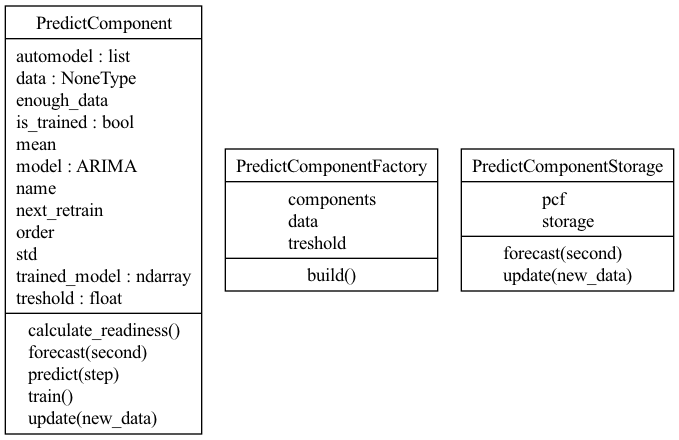
\includegraphics[width=0.8\textwidth]{chapter-4/predictor.png}
    \caption{Spesifikasi Kelas Penyusun Komponen \textit{Predictor}}
    \label{fig:predictor-spek}
\end{figure}

Secara umum, spesifikasi kelas bisa dilihat pada gambar \ref{fig:predictor-spek}. Kelas \textbf{\textit{Predict Component Storage}} akan membutuhkan \textbf{\textit{Predict Component Factory}} untuk membangun semua \textbf{\textit{Predict Component}} untuk setiap variabel yang ada. Setelah itu, terdapat operasi seperti meneruskan penambahan data serta meminta data prediksi ke setiap \textbf{\textit{Predict Component}}. Kelas ini akan digunakan oleh komponen \textbf{\textit{Flexible Control}} untuk lebih lanjutnya.